\chapter{Modello Entity Relationship - ER}
In questa parte si studierà la come progettare una base di dati a livello concettuale
e logico, partendo dai requisiti di utente.
Per capirne l'importanza è utile analizzare il ciclo di vita di un sistema informativo
\section{Fasi del ciclo di vita}
\begin{itemize}
    \item Studio di fattibilità: definizione costi e priorità
    \item Raccolta e analisi dei requisiti: studio delle proprietà del sistema
    \item Progettazione: di dati e funzioni
    \item Implementazione: realizzazione
    \item Validazione e collaudo: sperimentazione
    \item Funzionamento: il sistema diventa operativo
\end{itemize}
Il ciclo di vita segue un modello a spirale.
Per garantire prodotti di buona qualità è fondamentale seguire una metodologia
di progetto.
\paragraph*{Metodologia} è un'articolazione in fasi/passi di guida ad una attività di
progettazione.
Avere una metodologia di progetto:
\begin{itemize}
    \item Permette di suddividere la progettazione in fasi
    \item Fornisce una strategia da seguire
    \item Fornisce modelli di riferimento (linguaggi) per descrivere la realtà
    che stiamo progettando
\end{itemize}
Serve per garantire:
\begin{itemize}
    \item Generalità rispetto ai problemi da affrontare
    \item Qualità in termini di correttezza, completezza ed efficienza
    \item Facilità d'uso
\end{itemize}
La metodologia di basa su un principio semplice ma efficace:
\paragraph*{Separazione netta tra decisioni relative a:}
\begin{itemize}
    \item Cosa rappresentare 
    \item Come farlo
\end{itemize}
\section{La progettazione di basi di dati}
La progettazione si divide in 3 fasi:
\begin{itemize}
    \item Progettazione concettuale
    \item Progettazione logica
    \item Progettazione fisica
\end{itemize}
Ognuna delle fasi si basa su un modello, che permette di generare una rappresentazione
formale (schema) della base di dati ad un dato livello di astrazione (concettuale, logico, fisico).
\subsection{Progettazione concettuale}
Traduce i requisiti del sistema informatico in una descrizione formalizzata, integrata
delle esigenze aziendali, espressa in modo \textbf{indipendente} dalle scelte implementative.

\begin{itemize}
    \item Formale - Espressa con un linguaggio non ambiguo e capace di descrivere
    il sistema analizzato
    \item Integrata - Deve essere in grado di descrivere nella globalità l'ambiente analizzato
    \item Indipendete dall'ambiente tecnologico
\end{itemize}
\paragraph*{Nel nostro caso:}
\begin{itemize}
    \item Schema concettuale - \textbf{Modello ER}
    \item Schema logico - \textbf{Modello relazionale}
\end{itemize}
\subsection{Vantaggi della progettazione concettuale}
Permette una descrizione dei dati indipendente dagli aspetti tecnologici con un
livello di astrazione intermedio fra utente e sistema. Prevale l'aspetto intensionale.
\\ Si tratta di una rappresentazione prevalentemente grafica. Utile per la documentazione.
\section{Modello Entità Relazione}
Il modello ER è un modello grafico semi-formale per la rappresentazione di schemi
concettuali. Si è ormai affermato come standard nelle metodologie di progetto e nei
sistemi Software di ausilio alla progettazione.
\section{I Costrutti del modello ER}
\begin{itemize}
    \item Entità
    \item Relazione
    \item Attributo semplice
    \item Atrributo composto
    \item Cardinalità
    \item Cardinalità di un Attributo
    \item Identificatore interno
    \item Identificatore esterno
    \item Generalizzazione
    \item Sottoinsieme
\end{itemize}

\subsection{Entità}
Classe di oggetti (fatti, persone, cose) della applicazione di interesse
con proprità comuni e con esistenza autonoma e della quale si vogliono
registrare fatti specifici.
\begin{center}
    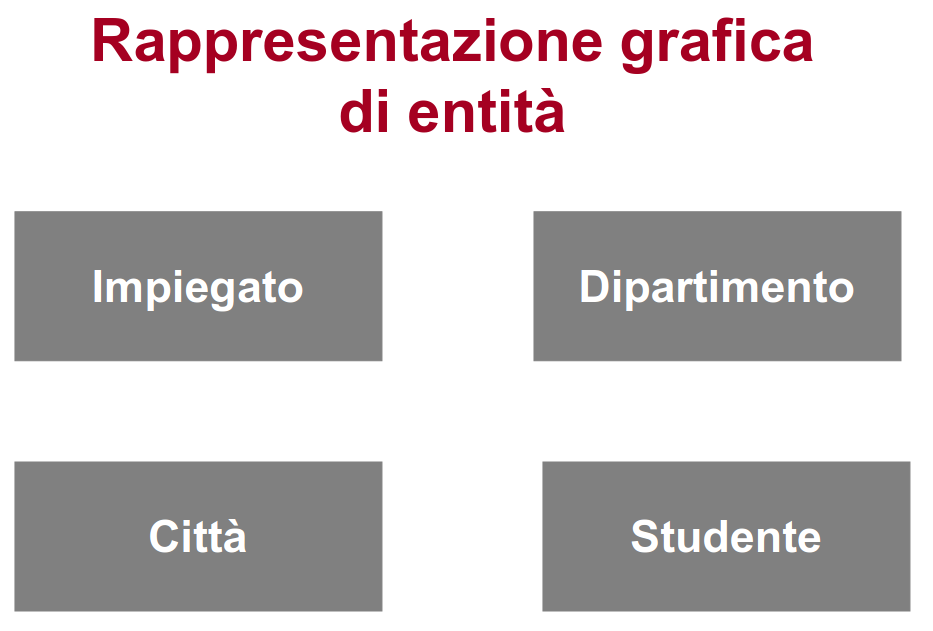
\includegraphics[width=100mm, scale=0.5]{rappresentazione_grafica_entita.png}
\end{center}
Definita come sostantivo al singolare (es. studente, classe, docente, ecc.)
A livello estensionale un'entità è costituira da un insieme di oggetti 
che sono chiamati le sue istanze.
\paragraph*{Istanza}
Occorrenza di un'entità, è l'oggetto della classe che entità rappresenta. Nello schema
concettuale rappresentiamo le entità, non le singole istanze.
\\ Riassumendo:
\begin{itemize}
    \item Conoscenza Astratta $\rightarrow$ Entità
    \item Conoscenza Concreta $\rightarrow$ Istanza di entità
\end{itemize}
\subsection*{Attributi}
Un attributo di un entità è una proprietà locale di un'entità di interesse ai
fini dell'applicazione. Associa ad ogni istanza di un'entità un valore appartenente
a un insieme detto dominio dell'attributo (es. int, string, char, ecc.).
\\ Viene definito quando si vuole rappresentare una proprietà locale
delle istanze dell'entità E.
\\ Una proprietà di un oggetto si dice locale quando in ogni istanza dello schema il valore
di tale proprietà dipende solamente dall'oggetto stesso e non ha alcun rapporto
con altri elementi dell'istanza dello schema.
\paragraph*{Attributi composti}
Si ottengono raggruppando attributi di una medesima entità o relazione che
presentano affinità nel loro significato o uso.
\paragraph*{Esempio:} Indirizzo è composto da Via, Numero, Cap.
\subsection*{Relazione-Associazione}
Ogni relazione ha un nome che la identifica univocamente nello schema.
\paragraph*{Convenzioni}
\begin{itemize}
    \item Singolare
    \item Sostantivi invece che verbi
\end{itemize}
A livello estensionale una relazione R tra le entità E ed F è costituita da un
insieme di coppie (x, y) tali che x è una istanza di E, ed y è un'istanza di F.
Ogni coppia è detta istanza della relazione R.
\\ Ciò significa che se in uno schema S è definita una relazione R sulle entità E ed F
\paragraph*{Istanze di associazione}
Combinazione (aggregazione) di istanze di entità che prendono parte alla associazione.
\paragraph*{Esempio:} Rossi insegna Basi di Dati
\subsection*{Osservazione importante}
Dalla semantica delle relazioni segue immediatamente che non posson oesistere due
istsanze della stessa relazione che coinvolgono le stesse istanze di entità.
\\ Due entità possono essere coinvolte in più relationship.
\\ Le relationship possono coinvolgere più di due entità.
\externaldocument[2-Rel]{2-Modello-Relazionale}
\paragraph*{Osservazione sul concetto di relazione} Il concetto di relazione sarà
spiegato meglio nel capitolo 2-Modello-Relazionale.
%Far funzionare link tra 2 diversi file
